% !TEX program = pdflatex
\documentclass{article}
\usepackage{tikz}

\begin{document}
\section*{Two impressions of one stamp}
\begin{figure}[ht]\centering
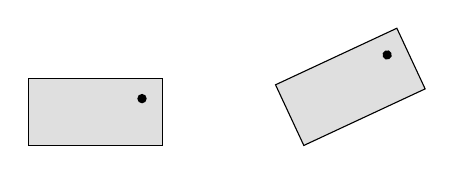
\begin{tikzpicture}

\foreach \offset/\turn in {0/0,3.5/25}{
 \begin{scope}[xshift=\offset cm,rotate=\turn,scale=.85]
 \filldraw[fill=gray!25] (0,0) rectangle (2,1);
 \fill (1.7,.7) circle (2pt);
 \end{scope}}
\end{tikzpicture}\caption{The dot identifies the same corner after rotation.}\end{figure}
\end{document}
